\subsection{实验目的-分析 oracle 日志}
分析 oracle 日志.
%
\subsection{实验原理}
\subsubsection{Oracle 加密原理}
当 Oracle 发起连接后,Oracle 客户端向 oracle 数据库发送自己版本号、
包含的加密算法等信息。最终服务端确定使用什么加密算法,
然后进行 O3logon 验证。O3logon 验证是一种查询-响应协议,
它利用 DES 加密技术保护这个会话的密钥(sesskey),
保证 sesskey 不会在网络中传输,所以即使有人监听网络也不会暴露核心密钥。
其中 O3logon 验证的核心是 sesskey。

Oracle 11g 在 10g 的基础上进行了一定的改变。假设我们已经取得一个含有 Oracle 登录信息的
网络通讯包。省略掉前面和密码关系不大的信息在数据包中寻找到 4 个相关信息,分别是数据库
发送给客户端的 S\_AUTH\_SESSKEY、AUTH\_VFR\_DATA、
客户端发送给服务器的 C\_AUTH\_SESSKEY 和 AUTH\_PASSWORD。

假设取得了 Oracle\_hash,11g 基本同于 10g,客户端和数据库分别以 Oracle\_hash 为基础生成
S\_AUTH\_SESSKEY 和 C\_AUTH\_SESSKEY。
客户端对传过来的 S\_AUTH\_SESSKEY 做 AES192 解密处理拿到
server\_sesskey,把 server\_sesskey 和自己的 client\_sesskey 做 md5 生成 combine,
用 combine 生成 AUTH\_PASSWORD。服务器最后用 combine 对
AUTH\_PASSWORD 解密,对比密码,如果密码一致则登陆成功。

11g 最大的变化在生成 Oracle\_hash 上采取了和 10g 不同的策略。Oracle 11g 为了提高
Oracle\_hash 的安全性,引入了 AUTH\_VFR\_DATA 这个随机值,
取消了明文密码。每个会话的 AUTH\_VFR\_DATA 都不同。从根本上避免 9i、10g
同字符串(用户名+密码组成的字符串)带来的无论哪台机器
oracle\_hash 一致的巨大安全隐患。
从 11g 开始,oracle 和密码相关登陆信息全部采用了密文。
有效地加大了破解难度。对于 oracle 安全性问题,
一定注意防止网络监听,设计 SID 的时候尽量避免 ORACLE、TEST 等常用名。
端口号尽量不要选用 1521 和 1523 来增加扫描难度。
使用复杂密码,定期更换密码等都会有助于 oracle 的安全
%
\subsubsection{Orabrute}
这里我们使用 Orabrute 工具来进行远程破解 oracle,
在使用这个工具的时候,需要系统提前安装好 sqlplus,
该工具的原理很简单,就是不停的调用 sqlplus 然后进行登录验证,
帐户选择的是 sys,密码则为 password.txt 中的密码单词。
只要登录成功 ,就会调用 selectpassword.sql 脚本抓取出
在 SYS.USER\$ 表中的其他用户的哈希值,然后退出程序。
这里有个值得注意的地方,当第二次运行 Orabrute 的时候,
需要删除或移动同目录下的前一次运行 Orabrute 时生成的
thepasswordsarehere.txt 文件。
%
\subsubsection{SQLPLUS}
Oracle 的 sqlplus 是与 oracle 数据库进行交互的客户端工具,
借助 sqlplus 可以查看、修改数据库记录。
在 sqlplus 中,可以运行 sqlplus 命令与 sql 语句。
%
\subsection{实验环境}
\begin{itemize}
  \item Windows server 2003: 192.168.1.2 wireshark、orabrute、sqlplus
  \item Windows server 2008 R2:192.168.1.3oracle 11g
\end{itemize}
%
\subsection{实验步骤}
\subsubsection{破解 oracle 用户 sys 的密码}
为了更直观地查看日志,在 Windows server 2008 R2 上,
单击``开始'' $ \rightarrow $ ``管理工具'' $ \rightarrow $
``事件查看器'',展开``Windows 日志'',右键``应用程序'',选择清除日志。
\begin{figure}[H]
  \begin{center}
    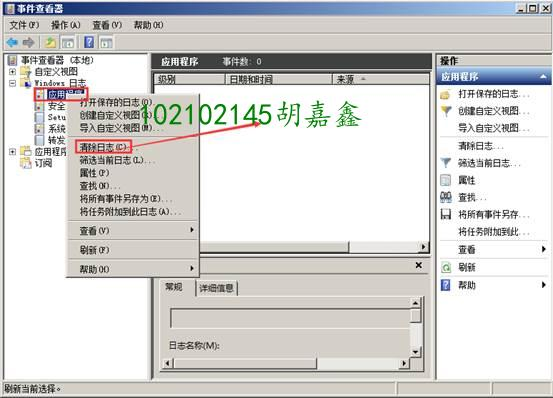
\includegraphics[width=0.40\textwidth]{2_14_1.jpeg}
  \end{center}
\end{figure}

在 Windows server 2003(\texttt{192.168.1.2})上打开 wireshark,
选择要监听的网卡后,单击``Start''按钮,开始进行抓包。
\begin{figure}[H]
  \begin{center}
    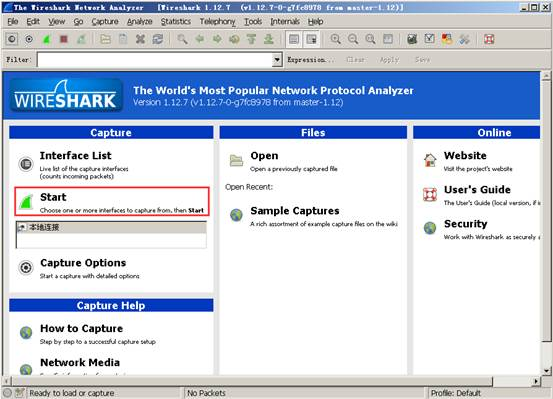
\includegraphics[width=0.40\textwidth]{2_14_2.jpeg}
  \end{center}
\end{figure}

事先先删除桌面上 \texttt{tools/oracle} 目录下的
thepasswordsarehere .txt 文件,没有则跳过。

打开 cmd,输入命令
\begin{minted}[bgcolor=bg,breaklines=true]{sh}
cd 'C:\Documents and Settings\Administrator\桌面\tools\oracle'
\end{minted}
再输入命令
\begin{minted}[bgcolor=bg,breaklines=true]{sh}
orabrute 192.168.1.3 1521 orcl 10 | more
\end{minted}
在破解过程中,可安空格键查看之后的内容。
\begin{figure}[H]
  \begin{center}
    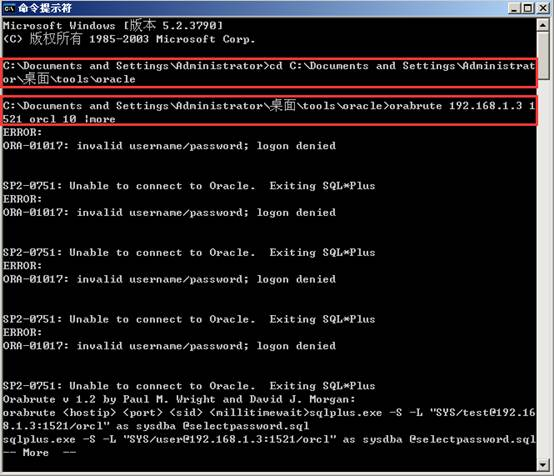
\includegraphics[width=0.40\textwidth]{2_14_3.jpeg}
  \end{center}
\end{figure}

除了在 cmd 中可以查看到破解结果,还可以在 thepasswordsare.txt 文件
中进行查看,可以看到 sys 破解出来的密码。
\begin{figure}[H]
  \begin{center}
    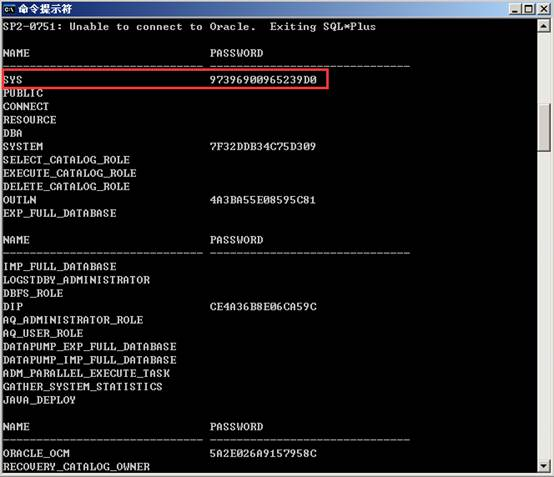
\includegraphics[width=0.40\textwidth]{2_14_4.jpeg}
  \end{center}
\end{figure}
\begin{figure}[H]
  \begin{center}
    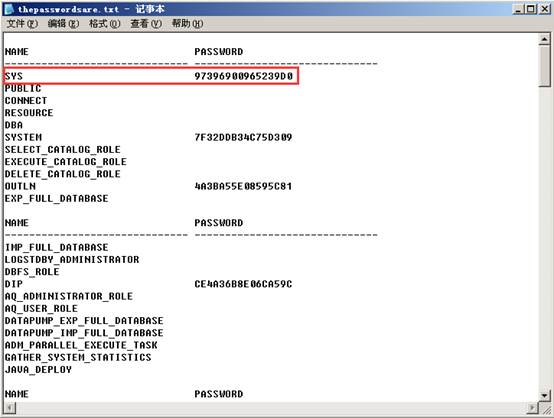
\includegraphics[width=0.40\textwidth]{2_14_5.jpeg}
  \end{center}
\end{figure}

打开 cain,在 Cracker 下选择 Oracle Hashs,
先在空白处单击一下鼠标,再单击``+''添加信息,
用户名为 sys,hash 值为 97396900965239D0,
单击``OK''。
\begin{figure}[H]
  \begin{center}
    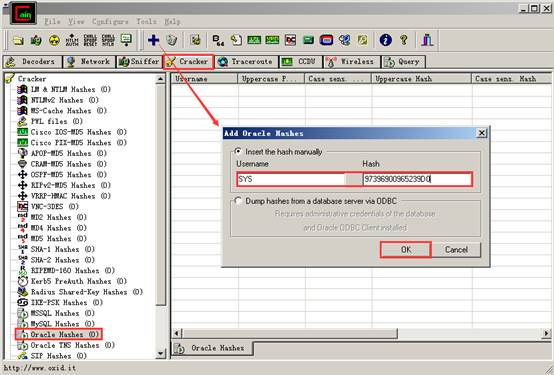
\includegraphics[width=0.40\textwidth]{2_14_6.jpeg}
  \end{center}
\end{figure}

右键添加的条目,选择
``Dictionary Attack''$ \rightarrow $``UPPRECASE Hashs''。
\begin{figure}[H]
  \begin{center}
    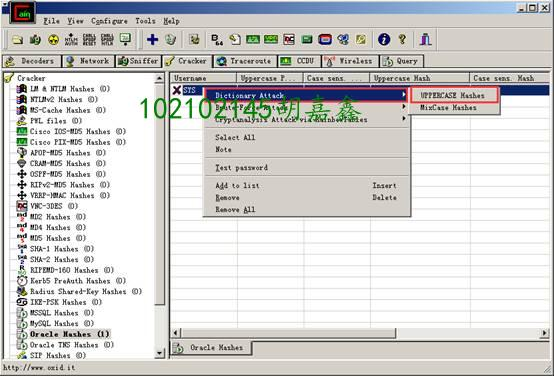
\includegraphics[width=0.40\textwidth]{2_14_7.jpeg}
  \end{center}
\end{figure}

在 Dictionary 下方的空白处右键,选择
``Add to list'',添加字典文件后,单击``Start'' 按钮,开始破解。
\begin{figure}[H]
  \begin{center}
    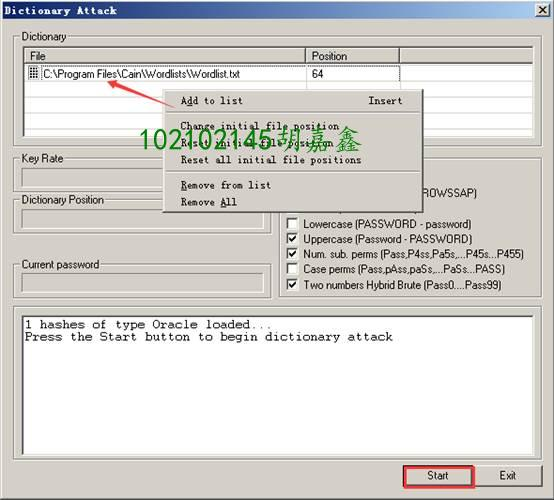
\includegraphics[width=0.40\textwidth]{2_14_8.jpeg}
  \end{center}
\end{figure}

破解出 sys 的密码为 Simplexue123(这里显示的时候不区分大小写)。
\begin{figure}[H]
  \begin{center}
    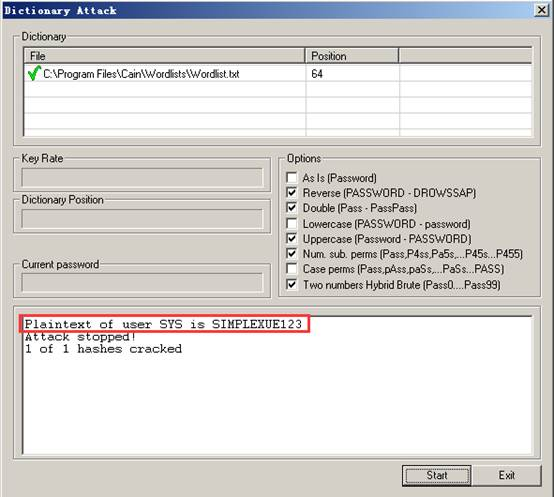
\includegraphics[width=0.40\textwidth]{2_14_9.jpeg}
  \end{center}
\end{figure}
%
\subsubsection{理解 oracle 数据库的破解过程}
Wireshark 停止抓包,过滤端口号为 1521 的数据包。
\begin{figure}[H]
  \begin{center}
    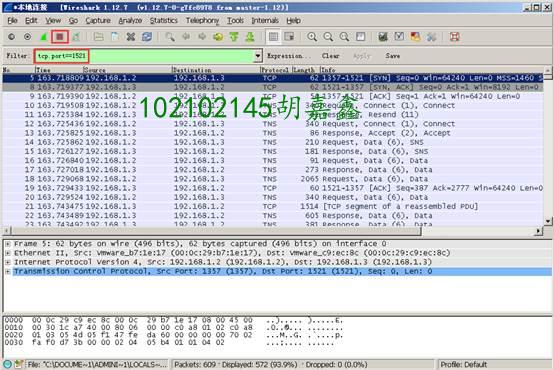
\includegraphics[width=0.40\textwidth]{2_14_10.jpeg}
  \end{center}
\end{figure}

下面我们对其中一个过程的数据包进行分析。首先查看第一个数据包,
源地址为 \texttt{192.168.1.2},源端口为 1357,
目的地址为 \texttt{192.168.1.3},目的端口为 1521,
TCP 序号为 SYN,且置为 1,
表示客户端 \texttt{192.168.1.2} 向服务器 \texttt{192.168.1.3} 发送了一个连接请求报文。
\begin{figure}[H]
  \begin{center}
    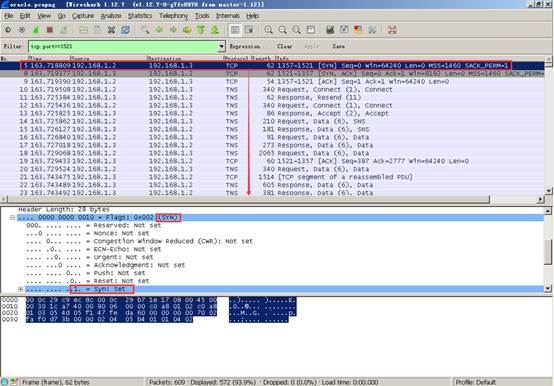
\includegraphics[width=0.40\textwidth]{2_14_11.jpeg}
  \end{center}
\end{figure}

再查看第二个数据包,\texttt{192.168.1.3} 收到请求后确认联机信息,
向 \texttt{192.168.1.2} 发送数据包,
SYN 置为 1,ACK 也置为 1。
\begin{figure}[H]
  \begin{center}
    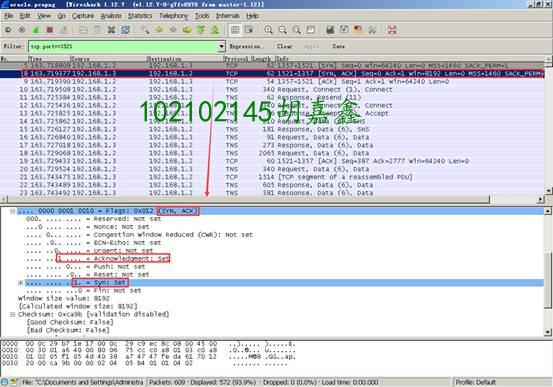
\includegraphics[width=0.40\textwidth]{2_14_12.jpeg}
  \end{center}
\end{figure}

查看第三个数据包,主机 \texttt{192.168.1.2} 收到数据包后检查无误,
向 \texttt{192.168.1.3} 发送数据包,
ACK 置为 1,至此三次握手完毕,连接建立。
\begin{figure}[H]
  \begin{center}
    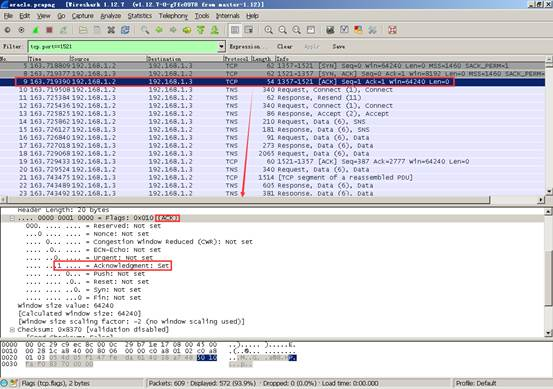
\includegraphics[width=0.40\textwidth]{2_14_13.jpeg}
  \end{center}
\end{figure}

在 TNS(Transparent Network Substrate Protocol)协议中,
每个 TNS 完整数据都包含一个通用包头,
说明接受数据的长度及其相关校验和解析的信息,类型 type 的值为 1 时,即
\texttt{Connect(1)},表示请求连接。
\begin{figure}[H]
  \begin{center}
    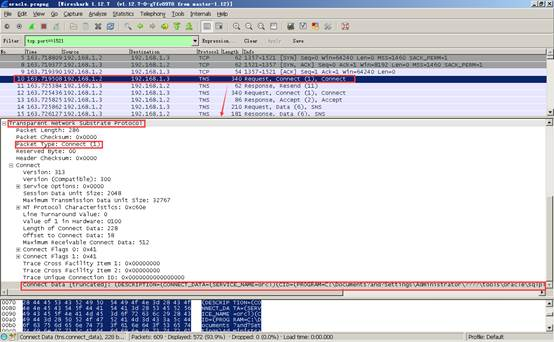
\includegraphics[width=0.40\textwidth]{2_14_14.jpeg}
  \end{center}
\end{figure}

当 type 的值为 11,即 \texttt{Resend(11)} 时,表示重新发送,
即服务器要求客户端再发送一次连接请求。
\begin{figure}[H]
  \begin{center}
    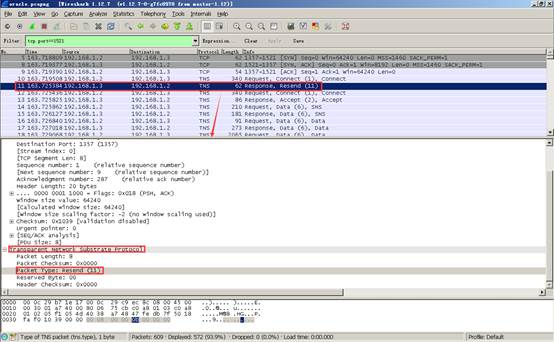
\includegraphics[width=0.40\textwidth]{2_14_15.jpeg}
  \end{center}
\end{figure}

客户端再次发送连接请求。当 type 的值为 2,
即 \texttt{Accept(2)} 时,表示接受。
\begin{figure}[H]
  \begin{center}
    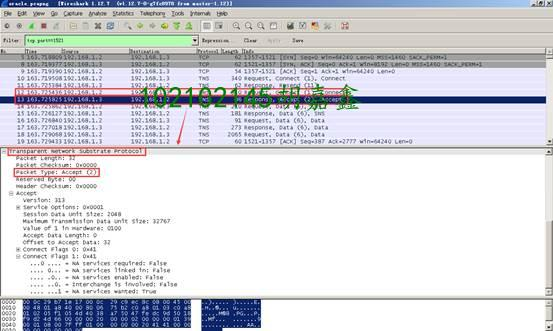
\includegraphics[width=0.40\textwidth]{2_14_16.jpeg}
  \end{center}
\end{figure}

当 type 的值为 6,即 \texttt{Data(6)} 时,表示数据,
即进行着数据的传输。继续往下分析数据包,
我们找到相关的登录请求信息数据包,我们发现无法看到明文密码,
因为 oracle 的登录认证过程密码是加密的,无法查看。
\begin{figure}[H]
  \begin{center}
    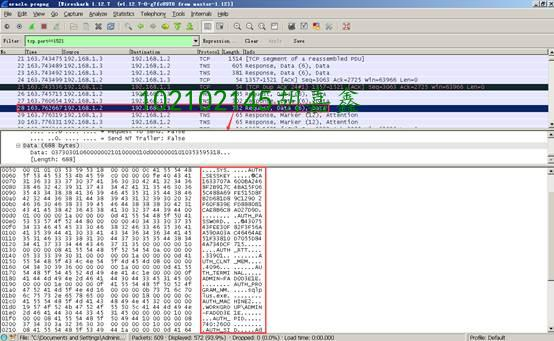
\includegraphics[width=0.40\textwidth]{2_14_17.jpeg}
  \end{center}
\end{figure}

登录失败信息如下。
\begin{figure}[H]
  \begin{center}
    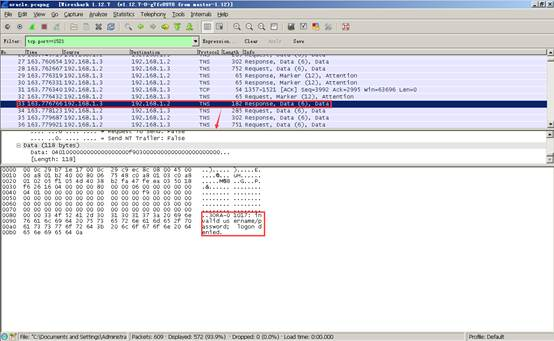
\includegraphics[width=0.40\textwidth]{2_14_18.jpeg}
  \end{center}
\end{figure}

在抓取的破解数据包中,有这样一个数据包,通过分析,
可以发现这是登录成功时显示的信息,说明破解出了 sys 的密码,
登录成功了。
\begin{figure}[H]
  \begin{center}
    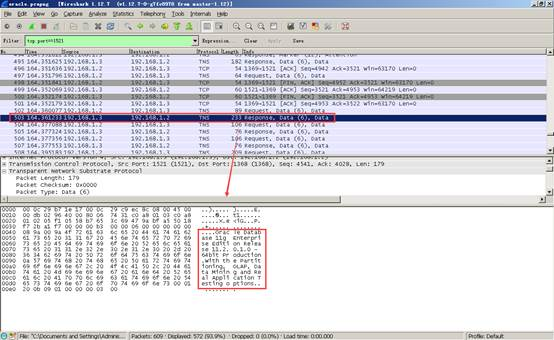
\includegraphics[width=0.40\textwidth]{2_14_19.jpeg}
  \end{center}
\end{figure}

登录成功后调用 selectpassword.sql 脚本,
执行 SQL 语句
\begin{minted}[bgcolor=bg,breaklines=true]{sql}
select name,password from sys.user$;
\end{minted}
抓取出在 SYS.USER\$ 表中的其他用户的哈希值,
并将结果保存在 \texttt{thepasswordsare.txt} 文件中,最后退出程序。
\begin{figure}[H]
  \begin{center}
    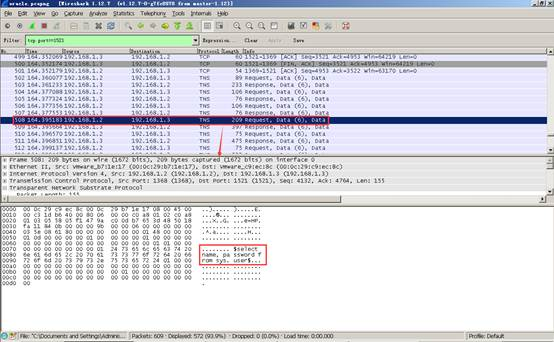
\includegraphics[width=0.40\textwidth]{2_14_20.jpeg}
  \end{center}
\end{figure}

\texttt{selectpassword.sql} 脚本内容如下。
\begin{figure}[H]
  \begin{center}
    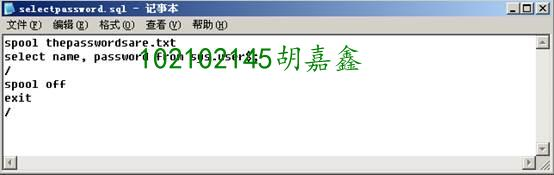
\includegraphics[width=0.40\textwidth]{2_14_21.jpeg}
  \end{center}
\end{figure}

所以,只要在破解过程中,有一个密码可以登录成功,
我们可以获得所有的用户名及其密码 hash 值,
再使用 cain 来破解密码。\texttt{thepasswordsare.txt} 的内容如下。
\begin{figure}[H]
  \begin{center}
    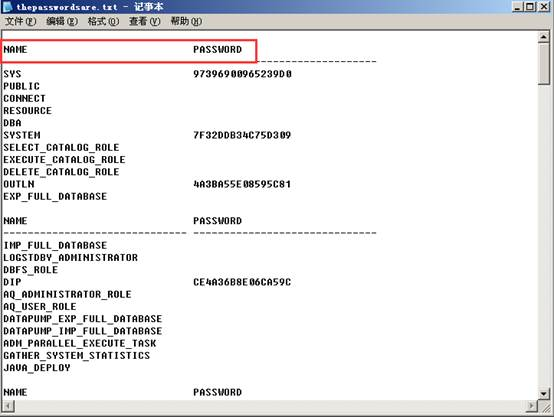
\includegraphics[width=0.40\textwidth]{2_14_22.jpeg}
  \end{center}
\end{figure}
%
\subsubsection{查看日志}
切换到 Windows server 2008 R2 上,打开 cmd,使用命令
\begin{minted}[bgcolor=bg,breaklines=true]{sh}
sqlplus sys/Simplexue123 as sysdba
\end{minted}
进入 oracl。

在 oracl 中,使用命令
\begin{minted}[bgcolor=bg,breaklines=true]{sh}
show parameter audit;
\end{minted}
查看和审计相关的主要参数,
audit\_sys\_operations 默认为 false,当设置为 true 时,
所有 sys 用户(包括以 sysdba,sysoper 身份登录的用户)的操作都会被记录,
audit trail 不会写在 aud\$表 中,
如果是 windows 平台,audit trail 会记录在 windows 的
事件管理中,如果是 linux/unix 平台则会记录在 audit\_file\_dest 参数指定的文件中。
所以本实验审计 sys 的信息时使用事件查看器进行查看。
\begin{figure}[H]
  \begin{center}
    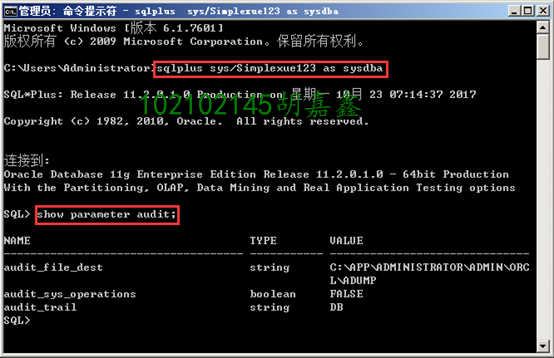
\includegraphics[width=0.40\textwidth]{2_14_23.png}
  \end{center}
\end{figure}

在 Windows server 2008 R2 上刷新``应用程序''日志。
\begin{figure}[H]
  \begin{center}
    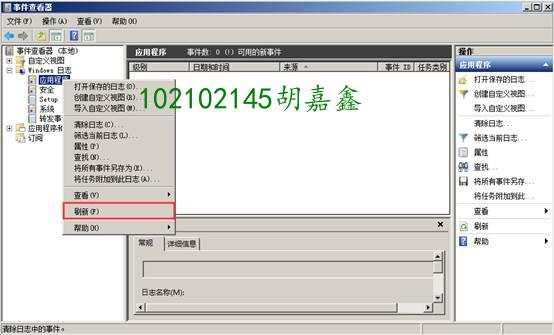
\includegraphics[width=0.40\textwidth]{2_14_24.jpeg}
  \end{center}
\end{figure}

发现有多条新增多条应用程序日志信息,查看某条信息记录。
\begin{figure}[H]
  \begin{center}
    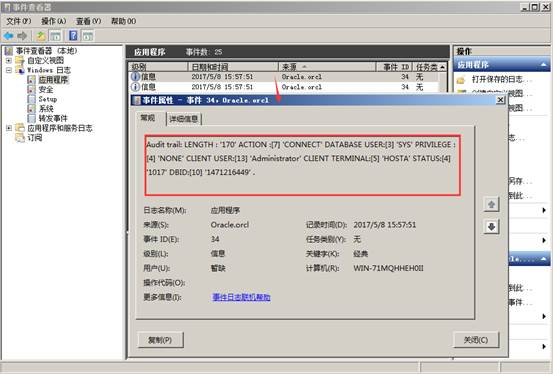
\includegraphics[width=0.40\textwidth]{2_14_25.jpeg}
  \end{center}
\end{figure}
\begin{figure}[H]
  \begin{center}
    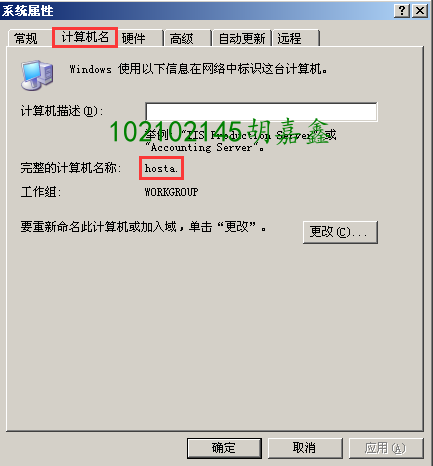
\includegraphics[width=0.40\textwidth]{2_14_26.png}
  \end{center}
\end{figure}

在查看这些消息记录时,发现有一条记录与其他的记录相比,
略有不同,\texttt{STATUS:[1] '0'}表示数据库连接成功。
在短时间内有大量的 oracle 数据库连接审计信息,在大多数连接失败的信息中,
有连接成功的记录,我们有理由相信数据库遭受到了暴力破解攻击。

这时我们就需要采取应对的应对措施。例如关闭数据库、更改数据库连接密码、
限制登录连接次数等等。
\begin{figure}[H]
  \begin{center}
    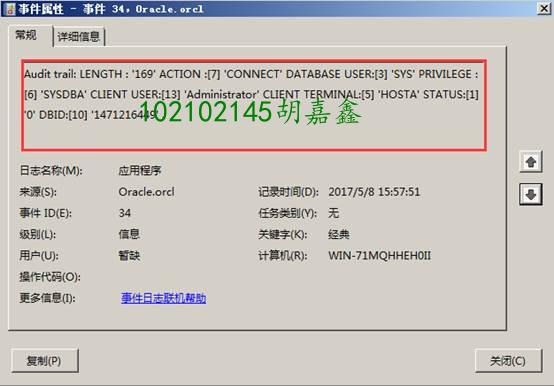
\includegraphics[width=0.40\textwidth]{2_14_27.jpeg}
  \end{center}
\end{figure}

再次清空``应用程序''日志。
在 Windows server 2003(\texttt{192.168.1.2})上,在 cmd 中输入命令
\begin{minted}[bgcolor=bg,breaklines=true]{sh}
sqlplus sys/Simplexue123@192.168.1.3:1521/orcl as sysdba
\end{minted}
使用破解出来的密码进行登录,登录成功。
\begin{figure}[H]
  \begin{center}
    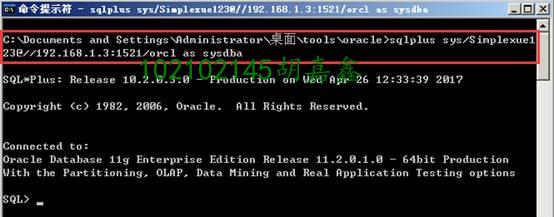
\includegraphics[width=0.40\textwidth]{2_14_28.jpeg}
  \end{center}
\end{figure}

在 Windows server 2008 R2(\texttt{192.168.1.3})上查看
``应用程序''日志,发现其信息与我们之前猜测的一样,
为登录成功的审计日志信息。
\begin{figure}[H]
  \begin{center}
    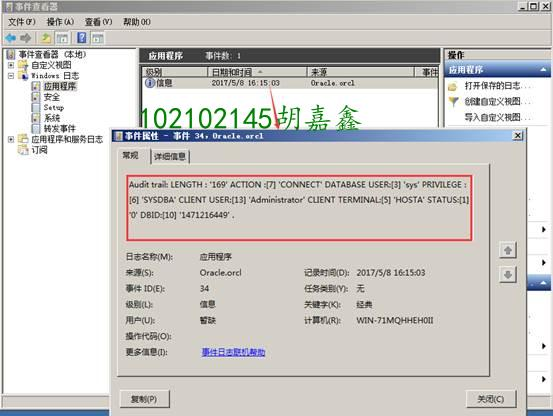
\includegraphics[width=0.40\textwidth]{2_14_29.jpeg}
  \end{center}
\end{figure}

Oracle 11g 中为了防止暴力破解数据库中用户的密码,
提供了一种常见手段:延长失败尝试响应。

这种手段的策略是:在连续使用错误密码反复尝试登录时,从第四次错误尝试开始,
每次增加 1 秒的延迟,最长延迟目前是 10 秒。

使用这种手段可以相对比较有效的防治用户密码的暴力破解
, 能够使用到这种手段的前提是 FAILED\_LOGIN\_ATTEMPTS 参数设置的足够
大或无限大,否则用户密码超过 10 次的错误尝试之后该用户将被锁定。

所以本实验为了演示效果较佳,使用的密码文件的密码数较少,便于破解。
